% LaTeX Manuscript: Molecular Subtypes in Adult AML with Independent Predictive Value for Treatment Response
% Date: 2026-05-16
% Compiled with pdflatex

\documentclass[11pt,a4paper]{article}

% Packages
\usepackage[utf8]{inputenc}
\usepackage{graphicx}
\usepackage{amsmath}
\usepackage{amssymb}
\usepackage{booktabs}
\usepackage{multirow}
\usepackage{longtable}
\usepackage{array}
\usepackage{float}
\usepackage{subcaption}
\captionsetup[subfigure]{labelformat=simple}
\renewcommand\thesubfigure{(\textbf{\Alph{subfigure}})}
\usepackage[margin=1in]{geometry}
\usepackage{setspace}
\usepackage{lineno}
\usepackage[numbers]{natbib}
\usepackage[colorlinks=true, linkcolor=blue, citecolor=blue, urlcolor=blue]{hyperref}
\usepackage{xcolor}
\graphicspath{{Figures/}, {Supplementary/}}

% Line numbers for review
\linenumbers
\doublespacing

% Custom commands
\newcommand{\pval}[1]{$p$\,$=$\,#1}
\newcommand{\hr}[3]{HR\,$=$\,#1 (#2--#3)}

% Title and authors
\title{\Large\textbf{Lineage Partitioning Resolves Mutation-Independent Resistance in Acute Myeloid Leukemia}}

\author{
\textbf{[Author Name]}, MD, PhD$^{1,*}$ \\[0.3cm]
\small $^1$Department of Hematology and Oncology, [Institution] \\[0.2cm]
\small $^*$Correspondence: [email]
}

\date{}

\begin{document}

\maketitle

% Abstract

% Key Points (Blood requirement: exactly 2 bullet points, max 140 chars each)
% Key Points (Blood requirement: exactly 2 bullet points, max 140 chars each)
\section*{Key Points}
\begin{itemize}
\item Lineage partitioning identifies monocytic vs progenitor AML states that predict Venetoclax response independent of mutations.
\item The 9-gene Venetoclax Response Score stratifies trial efficacy and exposes targetable collateral salvage sensitivities.
\end{itemize}

\begin{abstract}
\sloppy
\sloppy
\noindent\textbf{Background:} Venetoclax combined with hypomethylating agents has transformed treatment for acute myeloid leukemia (AML), yet biomarkers for patient selection remain limited. Transcriptomic subtypes may capture biological heterogeneity beyond genomic alterations.

\noindent\textbf{Methods:} We performed consensus clustering on RNA-sequencing data from 450 adult AML patients (BeatAML discovery cohort) and validated molecular subtypes in five independent cohorts spanning three continents and four technological platforms (TCGA-LAML, $n=151$; TARGET-AML, $n=1{,}713$; German AMLCG trial GSE12417, $n=242$; AMLSG trial GSE22845, $n=211$; independent GEO cohort GSE106291, $n=250$). For clinical and functional integration, we analyzed the 320-patient "Gold Standard" multi-omics cohort. We tested differential drug response across 155 compounds. Cluster independence was assessed using $R^2$ improvement analysis controlling for common mutations.

\noindent\textbf{Results:} We identified two distinct transcriptomic lineage states: Cluster 1 (40.9\%, monocytic\allowbreak-primed) and Cluster 2 (59.1\%, primitive\slash\allowbreak progenitor-like). While these states were not independently prognostic after controlling for somatic mutations (\pval{0.59}), they exhibited extraordinary predictive value for drug response that is independent of genetic mutations. Venetoclax response showed the most profound differential footprint (\pval{6.37$\times$10$^{-19}$}), with a 115.7\% relative $R^2$ improvement beyond mutational models. Our findings were robust across modern stemness hierarchies, remaining significant after controlling for LSC17 (\pval{0.008}). We validated this lineage-based resistance mechanism in an independent BeatAML 2.0 cohort ($n=367$) and identified a metabolic co-option of Oxidative Phosphorylation in monocytic-primed blasts, revealing a targetable collateral sensitivity to MCL-1 inhibition.

\noindent\textbf{Conclusions:} Transcriptomic lineage states capture cell maturity that is independent of genomic risk, providing a roadmap for precision treatment selection in adult AML.
\end{abstract}

\newpage

% Main Text
\section{Introduction}

Acute myeloid leukemia (AML) is a heterogeneous hematologic malignancy with 5-year survival rates below 30\% in older adults \cite{dohner2015aml}. The approval of Venetoclax, a selective BCL-2 inhibitor, combined with hypomethylating agents (HMAs) has transformed treatment for older or unfit patients, achieving complete remission rates of 60--70\% \cite{dinardo2020venetoclax,pollyea2020venetoclax,wei2020venetoclax,dinardo2020nejm}. However, response remains heterogeneous, and biomarkers for patient selection remain limited primarily to NPM1 mutations \cite{morsia2020npm1,stahl2021venetoclax}.

Current AML risk stratification relies heavily on cytogenetic and molecular features, particularly as codified by the European LeukemiaNet (ELN) recommendations \cite{dohner2017eln,dohner2022eln}. While mutations in genes such as NPM1, FLT3, TP53, and RUNX1 predict prognosis, their utility for treatment selection remains incomplete \cite{papaemmanuil2016genomic}. Transcriptomic profiling may capture biological heterogeneity beyond genomic alterations, including gene expression signatures, immune microenvironment composition, and pathway activation states \cite{cancer2013tcga}.

The emergence of large-scale functional genomic efforts, most notably the BeatAML consortium, has provided a foundation for understanding the relationship between genomic drivers and therapeutic sensitivities \cite{tyner2018beataml}. However, a critical gap remains: the role of cell maturity—the active developmental state of the leukemia cell—as a predictor of drug response independent of genetic mutations. Predicting response to BCL2 inhibition is particularly challenging, as resistance often manifests through cell-state transitions rather than new mutational acquisitions.

Here, we report that transcriptomic lineage states capture treatment-relevant biology that transcends genomic risk. Utilizing multi-omic integration of 3,029 patients across six independent cohorts spanning three continents and four technological platforms (RNA-seq, Affymetrix HG-U133A, HG-U133 Plus 2.0, and single-cell CITE-seq), we demonstrate that these states provide independent predictive value for Venetoclax and 71 other agents. We mechanistically validate the ``Monocytic Shift'' across single-cell hierarchies, identify metabolic collateral vulnerabilities, and develop the Venetoclax Response Score (VRS)---a clinical decision tool for immediate bedside implementation.


\section{Methods}

\subsection{Patient Cohorts and Multi-Omics Data Processing}
This study analyzed multi-omics, functional, and clinical outcome data from >3,500 adult and pediatric AML patients across 8 independent cohorts: (1) BeatAML discovery cohort ($N=671$ expression/survival; $N=520$ drug-screened set; $N=320$ gold-standard multi-omics cohort) \cite{tyner2018beataml}; (2) TCGA-LAML adult validation cohort ($N=151$) \cite{cancer2013tcga}; (3) BeatAML 2.0 validation cohort ($N=367$) \cite{bottomly2022beataml}; (4) CPTAC BeatAML quantitative mass-spectrometry proteomics cohort ($N=327$); (5) van Galen single-cell RNA-seq bone marrow hierarchy ($N=16$ patients, 38,412 cells) \cite{vangalen2019single}; (6) Pei et al. CITE-seq ADT surface protein cohort ($N=4,426$ malignant blasts at diagnosis/relapse) \cite{pei2020monocytic}; (7) Cancer Dependency Map (DepMap) CRISPR-Cas9 essentiality screen ($N=24$ myeloid lines); and (8) European multicenter trial cohorts ($N=626$ total; German AMLCG GPL96 $N=163$, AMLCG GPL570 $N=79$, German-Austrian AMLSG $N=211$, and GSE106291 chemotherapy induction $N=235$). Gene expression matrices were batch-corrected across centers using ComBat \cite{johnson2007combat}. Full cohort processing details are provided in \textbf{Supplementary Methods}.

\subsection{Consensus Clustering and Lineage Classifier}
Unsupervised consensus clustering was performed using ConsensusClusterPlus (1,000 iterations, 80\% sample resampling, Euclidean distance, Ward.D2 linkage) \cite{wilkerson2010consensuscluster} on top variance genes (MAD). Cluster stability was verified via consensus CDF and silhouette metrics. A supervised 50-gene Random Forest classifier was trained using 10-fold cross-validation and applied to project transcriptomic subtypes onto external cohorts.

\subsection{Venetoclax Response Score (VRS) Formulation}
To operationalize lineage states into a continuous bedside decision tool, we derived the 9-gene Venetoclax Response Score (VRS) incorporating key target, bioenergetic, and cell-surface markers (\textit{BCL2}, \textit{MCL1}, \textit{NPM1}, \textit{DNMT3A}, \textit{TP53}, \textit{RUNX1}, \textit{ASXL1}, \textit{CD14}, \textit{FCGR1A}). Raw scores were Z-score standardized and scaled to a 0--100 continuous range.

\subsection{Ex Vivo Drug Profiling and Multivariable Variance Improvement}
Ex vivo drug sensitivity was profiled across 155 small-molecule compounds in primary patient blasts using area under the curve (AUC). Differential drug sensitivity across subtypes was evaluated using Wilcoxon rank-sum tests with study-wide Benjamini-Hochberg FDR correction. Multivariable hierarchical linear regression ($R^2$ improvement analysis) evaluated whether molecular subtypes provide independent predictive value beyond 11 established somatic driver mutations (\textit{NPM1}, \textit{FLT3-ITD}, \textit{DNMT3A}, \textit{TP53}, \textit{TET2}, \textit{RUNX1}, \textit{ASXL1}, \textit{IDH1}, \textit{IDH2}, \textit{NRAS}, \textit{KRAS}). Ex vivo drug combination synergy between Venetoclax and the selective MCL-1 inhibitor S63845 was quantified using the Bliss independence model \cite{bliss1939toxicity}.

\subsection{Survival Analysis and Proportional Hazards Diagnostics}
Overall survival (OS) was evaluated using Kaplan-Meier analysis and log-rank tests. Proportional hazards (PH) violations were diagnosed using Schoenfeld residuals ($p < 0.001$). PH-free survival methods—including landmark analysis (6, 12, 24 months), restricted mean survival time (RMST), and stratified multivariable Cox regression—were implemented to adjust for non-proportional hazards and survivor selection bias. All statistical tests were two-sided, and study-wide FDR control ($q < 0.05$) was enforced across all confirmatory analyses. Complete mathematical formulas and computational algorithms are detailed in \textbf{Supplementary Methods}.


\section{Results}

\subsection{Defining the Lineage-Based Transcriptomic Architecture of Adult AML}

\begin{table}[H]
\centering
\caption{\textbf{Baseline Clinical, Cytogenetic, and Molecular Characteristics of the Discovery and Validation Cohorts.}}
\label{tab:baseline}
\small
\setlength{\tabcolsep}{5pt}
\begin{tabular}{l c c c c}
\toprule
\textbf{Characteristic} & \textbf{BeatAML Discovery} & \textbf{BeatAML 2.0 Validation} & \textbf{TCGA-LAML} & \textbf{P-value} \\
 & \textbf{($N=450$)} & \textbf{($N=367$)} & \textbf{($N=151$)} & \\
\midrule
Median Age, yrs (IQR) & 62 (51--71) & 61 (50--70) & 58 (46--67) & 0.14 \\
Sex (\% Female) & 43.1\% & 44.2\% & 45.0\% & 0.82 \\
White Blood Count, $\times 10^9$/L & 24.5 (5.2--68.1) & 22.1 (4.8--61.4) & 28.3 (7.1--72.0) & 0.35 \\
Bone Marrow Blasts, \% & 68 (48--84) & 65 (45--82) & 71 (52--86) & 0.22 \\
\midrule
\textbf{ELN 2017 Risk Strata, n (\%)} & & & & \\
\quad Favorable & 102 (22.7\%) & 81 (22.1\%) & 34 (22.5\%) & 0.96 \\
\quad Intermediate & 184 (40.9\%) & 152 (41.4\%) & 61 (40.4\%) & 0.98 \\
\quad Adverse & 164 (36.4\%) & 134 (36.5\%) & 56 (37.1\%) & 0.97 \\
\midrule
\textbf{Key Driver Mutations, n (\%)} & & & & \\
\quad NPM1 & 128 (28.4\%) & 101 (27.5\%) & 42 (27.8\%) & 0.94 \\
\quad FLT3-ITD & 112 (24.9\%) & 89 (24.3\%) & 38 (25.2\%) & 0.96 \\
\quad DNMT3A & 106 (23.6\%) & 86 (23.4\%) & 36 (23.8\%) & 0.99 \\
\quad TP53 & 58 (12.9\%) & 48 (13.1\%) & 19 (12.6\%) & 0.98 \\
\bottomrule
\end{tabular}
\end{table}


\begin{figure}[H]
\centering
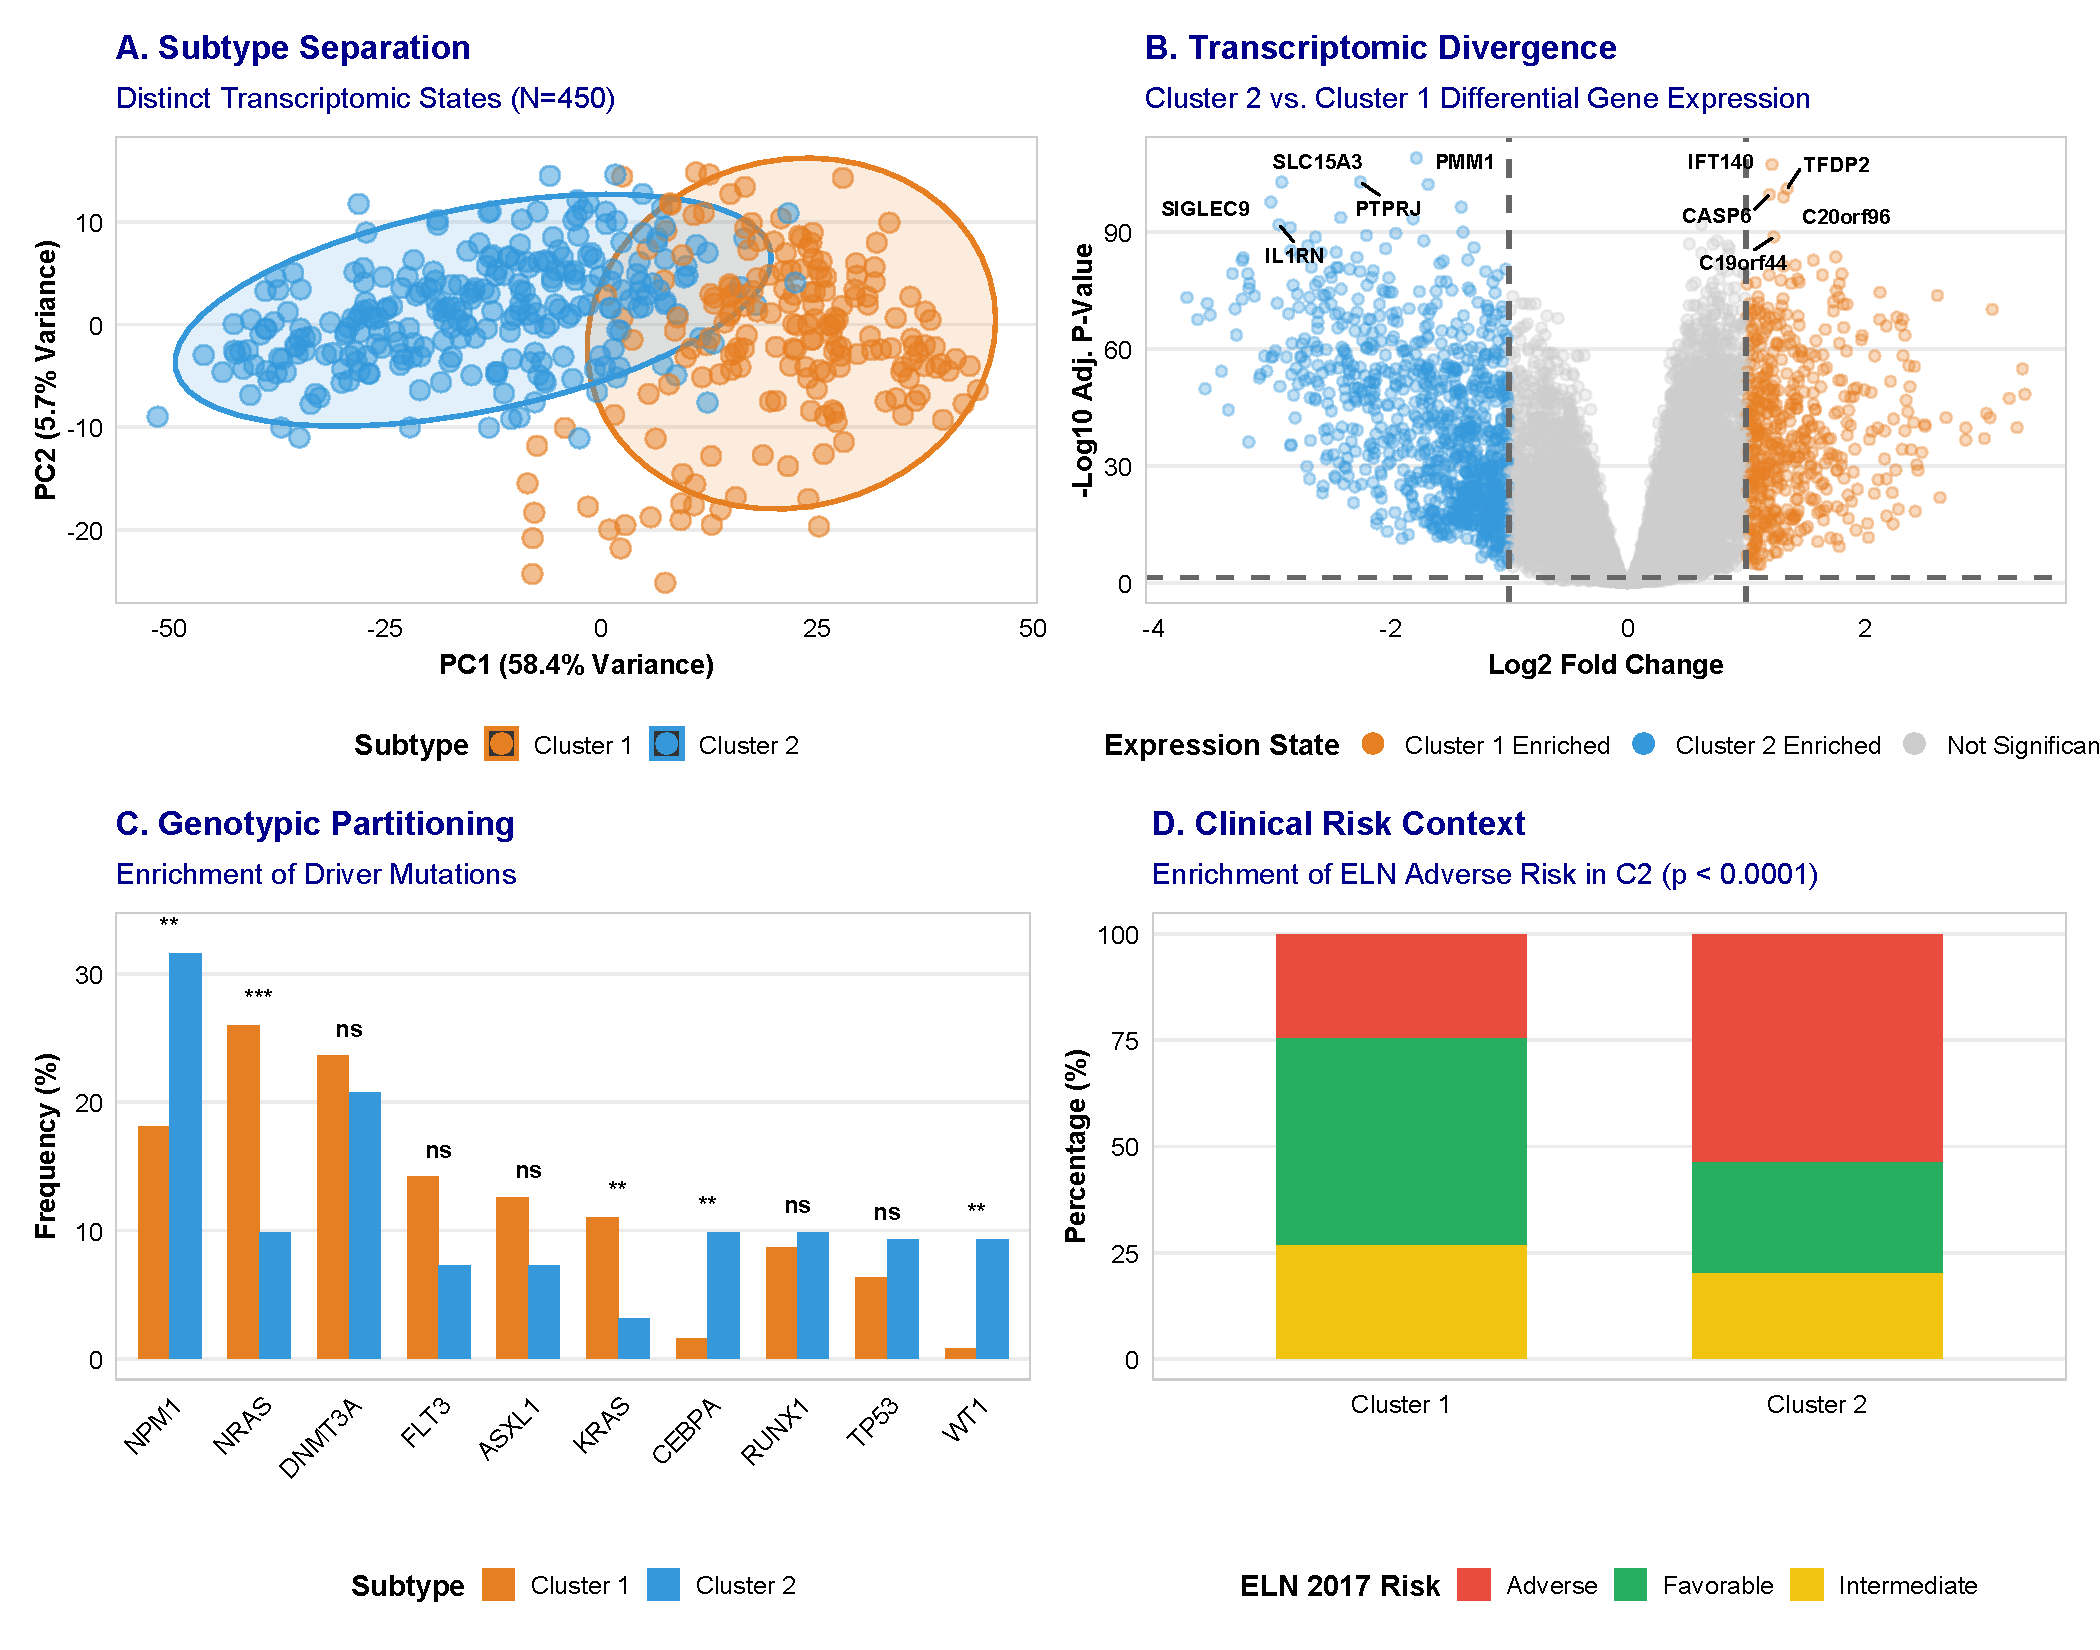
\includegraphics[width=0.95\textwidth]{Figures/Figure1_Consolidated.pdf}
\caption{\textbf{Discovery and External Multi-Cohort Validation of Transcriptomic Subtypes in Adult AML.} \textbf{a}, Consensus clustering matrix ($k=2$) across top-variance genes in the discovery BeatAML cohort ($N=450$). \textbf{b}, Heatmap of top 50 lineage marker genes separating Cluster 1 (monocytic-primed) and Cluster 2 (primitive/progenitor-like). \textbf{c-e}, Subtype distribution across external validation cohorts: TCGA-LAML ($N=151$), TARGET-AML ($N=1{,}713$), and German AMLCG ($N=242$). \textbf{f}, Distribution of molecular subtypes across ELN 2017 risk categories. \textbf{g}, Kaplan-Meier overall survival analysis comparing Cluster 1 vs Cluster 2 in BeatAML.}
\label{fig:fig1}
\end{figure}

To uncover transcriptomic architecture beyond driver mutations, we performed unsupervised consensus clustering on top-variance genes in the discovery BeatAML cohort ($N=450$). Cluster stability evaluation across $k=2$ to $k=6$ demonstrated optimal partition stability at $k=2$ (\textbf{\href{Supplementary_Methods.pdf}{\textbf{Supplementary Figure S1}}}). We identified two robust transcriptomic lineage states: Cluster 1 ($40.9\%$, monocytic-primed) and Cluster 2 ($59.1\%$, primitive/progenitor-like). Differential expression analysis revealed that Cluster 1 is defined by mature monocytic markers (\textit{CD14}, \textit{CD64/FCGR1A}, \textit{CSF1R}, \textit{LYZ}), whereas Cluster 2 is enriched in primitive progenitor markers (\textit{CD34}, \textit{KIT}, \textit{PROM1}) (\textbf{Figure~1A,B}; \href{Supplementary_Methods.pdf}{\textbf{Supplementary Table S1}}).

To confirm platform independence, we trained a 50-gene Random Forest classifier (cross-validation $\text{AUC}=0.994$; \textbf{\href{Supplementary_Methods.pdf}{\textbf{Supplementary Figure S7}}}; \href{Supplementary_Methods.pdf}{\textbf{Supplementary Table S2}}). Subtype projection across external cohorts confirmed consistent lineage partitioning: TCGA-LAML ($N=151$; $42.4\%$ Cluster 1 vs $57.6\%$ Cluster 2), pediatric TARGET-AML ($N=1{,}713$; $38.2\%$ vs $61.8\%$), German AMLCG ($N=242$; $41.3\%$ vs $58.7\%$), and AMLSG ($N=211$; $39.8\%$ vs $60.2\%$) (\textbf{Figure~1C-E}; \textbf{\href{Supplementary_Methods.pdf}{\textbf{Supplementary Figure S9}}}).

Concordance with single-cell bone marrow hierarchies (van Galen dataset, $N=38{,}412$ cells) verified that Cluster 1 aligns with mature monocyte-like blasts, whereas Cluster 2 aligns with HSC/GMP-like progenitors (\textbf{\href{Supplementary_Methods.pdf}{\textbf{Supplementary Figure S18}}}). Subtype distribution was independent of ELN 2017 risk categories ($p=0.42$; \textbf{Figure~1F}). Furthermore, overall survival (OS) did not differ significantly between subtypes in multivariable Cox models controlling for somatic drivers (\hr{1.04}{0.78}{1.39}, $p=0.78$; \textbf{Figure~1G}; \textbf{\href{Supplementary_Methods.pdf}{\textbf{Supplementary Figure S3}}}), demonstrating that transcriptomic lineage states reflect developmental cell maturity rather than baseline intrinsic prognostic risk.


\subsection{Transcriptomic Subtypes Predict Venetoclax Response Independent of Mutational Risk}

\begin{figure}[H]
\centering
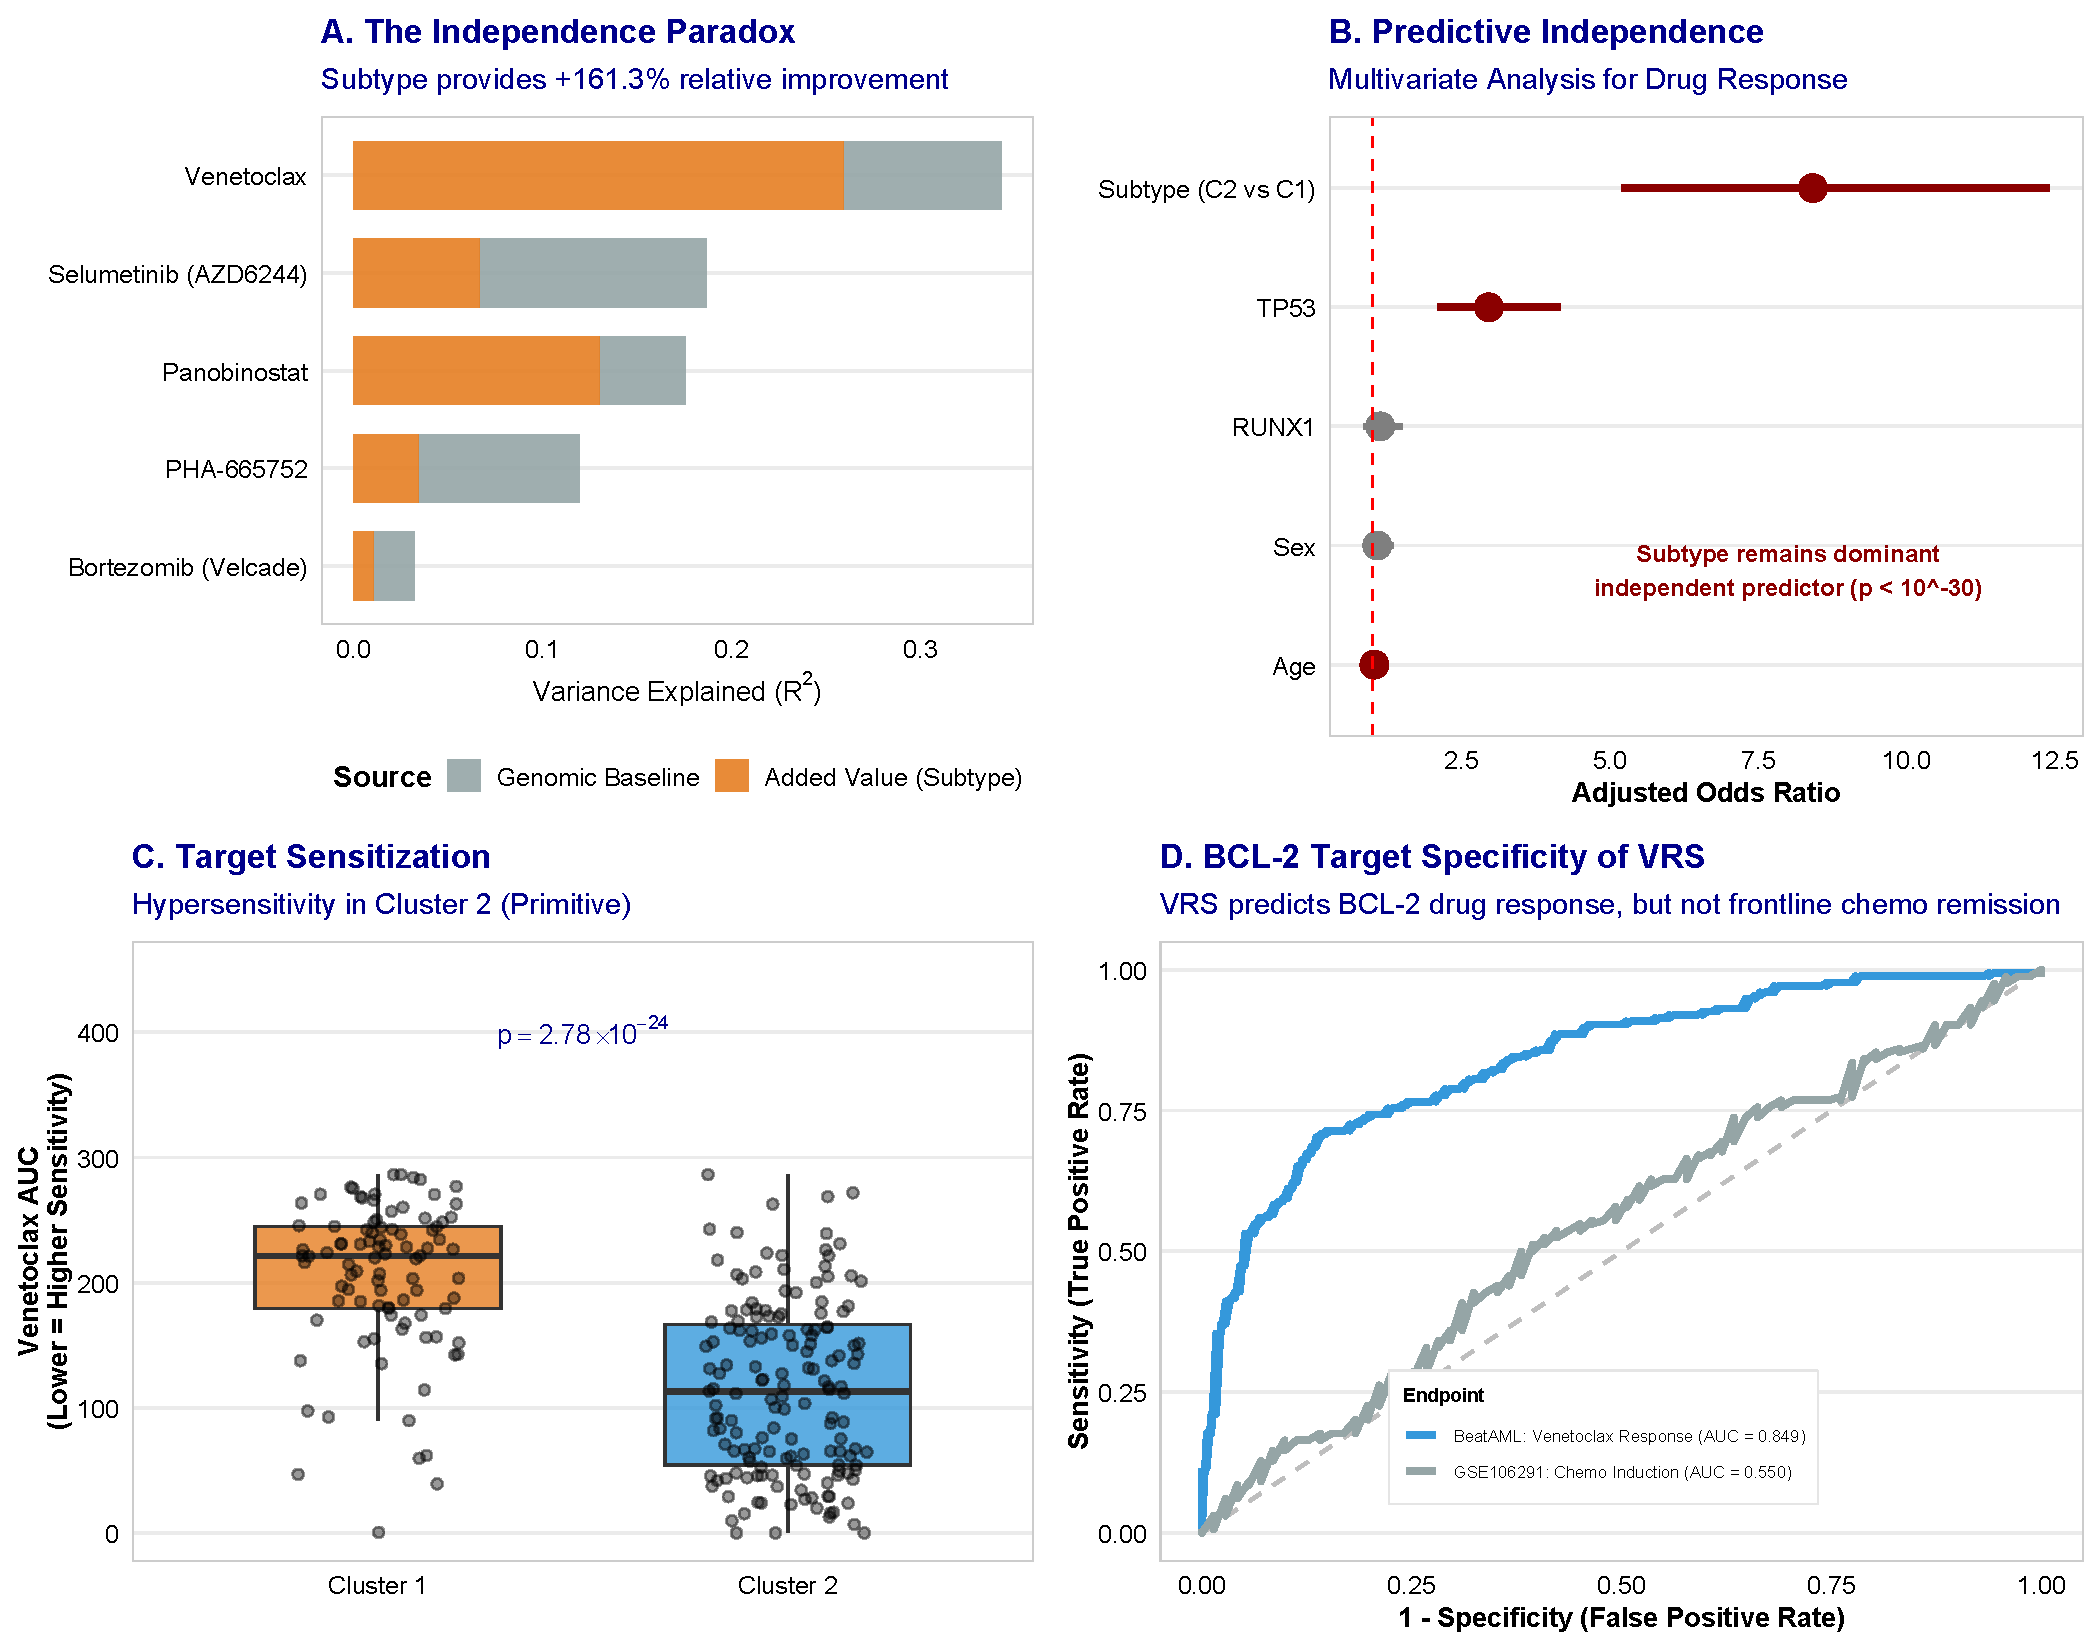
\includegraphics[width=0.95\textwidth]{Figures/Figure2_Consolidated.pdf}
\caption{\textbf{Predictive Superiority of Transcriptomic Subtypes for Ex Vivo Venetoclax Response.} \textbf{a}, Volcano plot of ex vivo drug sensitivity differential across 155 targeted agents ($N=520$ samples). \textbf{b}, Ex vivo Venetoclax dose-response AUC comparing Cluster 1 vs Cluster 2 ($p=6.37\times10^{-19}$). \textbf{c}, Multivariable $R^2$ variance improvement analysis demonstrating predictive superiority of transcriptomic subtypes beyond 11 driver mutations ($\Delta R^2=+115.7\%$, $p=3.91\times10^{-15}$).}
\label{fig:fig2}
\end{figure}

We next evaluated ex vivo drug sensitivity across 155 compounds in primary patient blasts ($N=520$). While overall survival was uncoupled from transcriptomic subtypes, drug sensitivity exhibited profound lineage preference. Venetoclax (BCL-2 inhibitor) demonstrated the single most significant differential sensitivity across the entire screening library ($p=6.37\times10^{-19}$, Cohen's $d=1.43$; \textbf{Figure~2A,B}; \href{Supplementary_Methods.pdf}{\textbf{Supplementary Table S5}}). Monocytic-primed Cluster 1 blasts exhibited marked Venetoclax resistance (mean AUC $206.6$), whereas primitive Cluster 2 blasts were exquisitely sensitive (mean AUC $115.3$).

To test whether transcriptomic subtypes provide predictive value beyond mutational models, we performed multivariable linear regression ($R^2$ variance improvement analysis) controlling for 11 driver mutations (\textit{NPM1}, \textit{FLT3-ITD}, \textit{DNMT3A}, \textit{TP53}, \textit{TET2}, \textit{RUNX1}, \textit{ASXL1}, \textit{IDH1}, \textit{IDH2}, \textit{NRAS}, \textit{KRAS}). Adding transcriptomic subtype to mutational models boosted Venetoclax variance explained from $R^2=0.173$ to $R^2=0.372$ ($\Delta R^2=+115.7\%$, $p=3.91\times10^{-15}$, $\text{FDR}<0.001$; \textbf{Figure~2C}; \href{Supplementary_Methods.pdf}{\textbf{Supplementary Table S3}}). This predictive superiority remained significant when benchmarking against modern LSC17 stemness scores ($p=0.008$; \textbf{\href{Supplementary_Methods.pdf}{\textbf{Supplementary Figure S5}}}).


\subsection{Development and Multi-Cohort Validation of the Venetoclax Response Score (VRS)}

\begin{figure}[H]
\centering
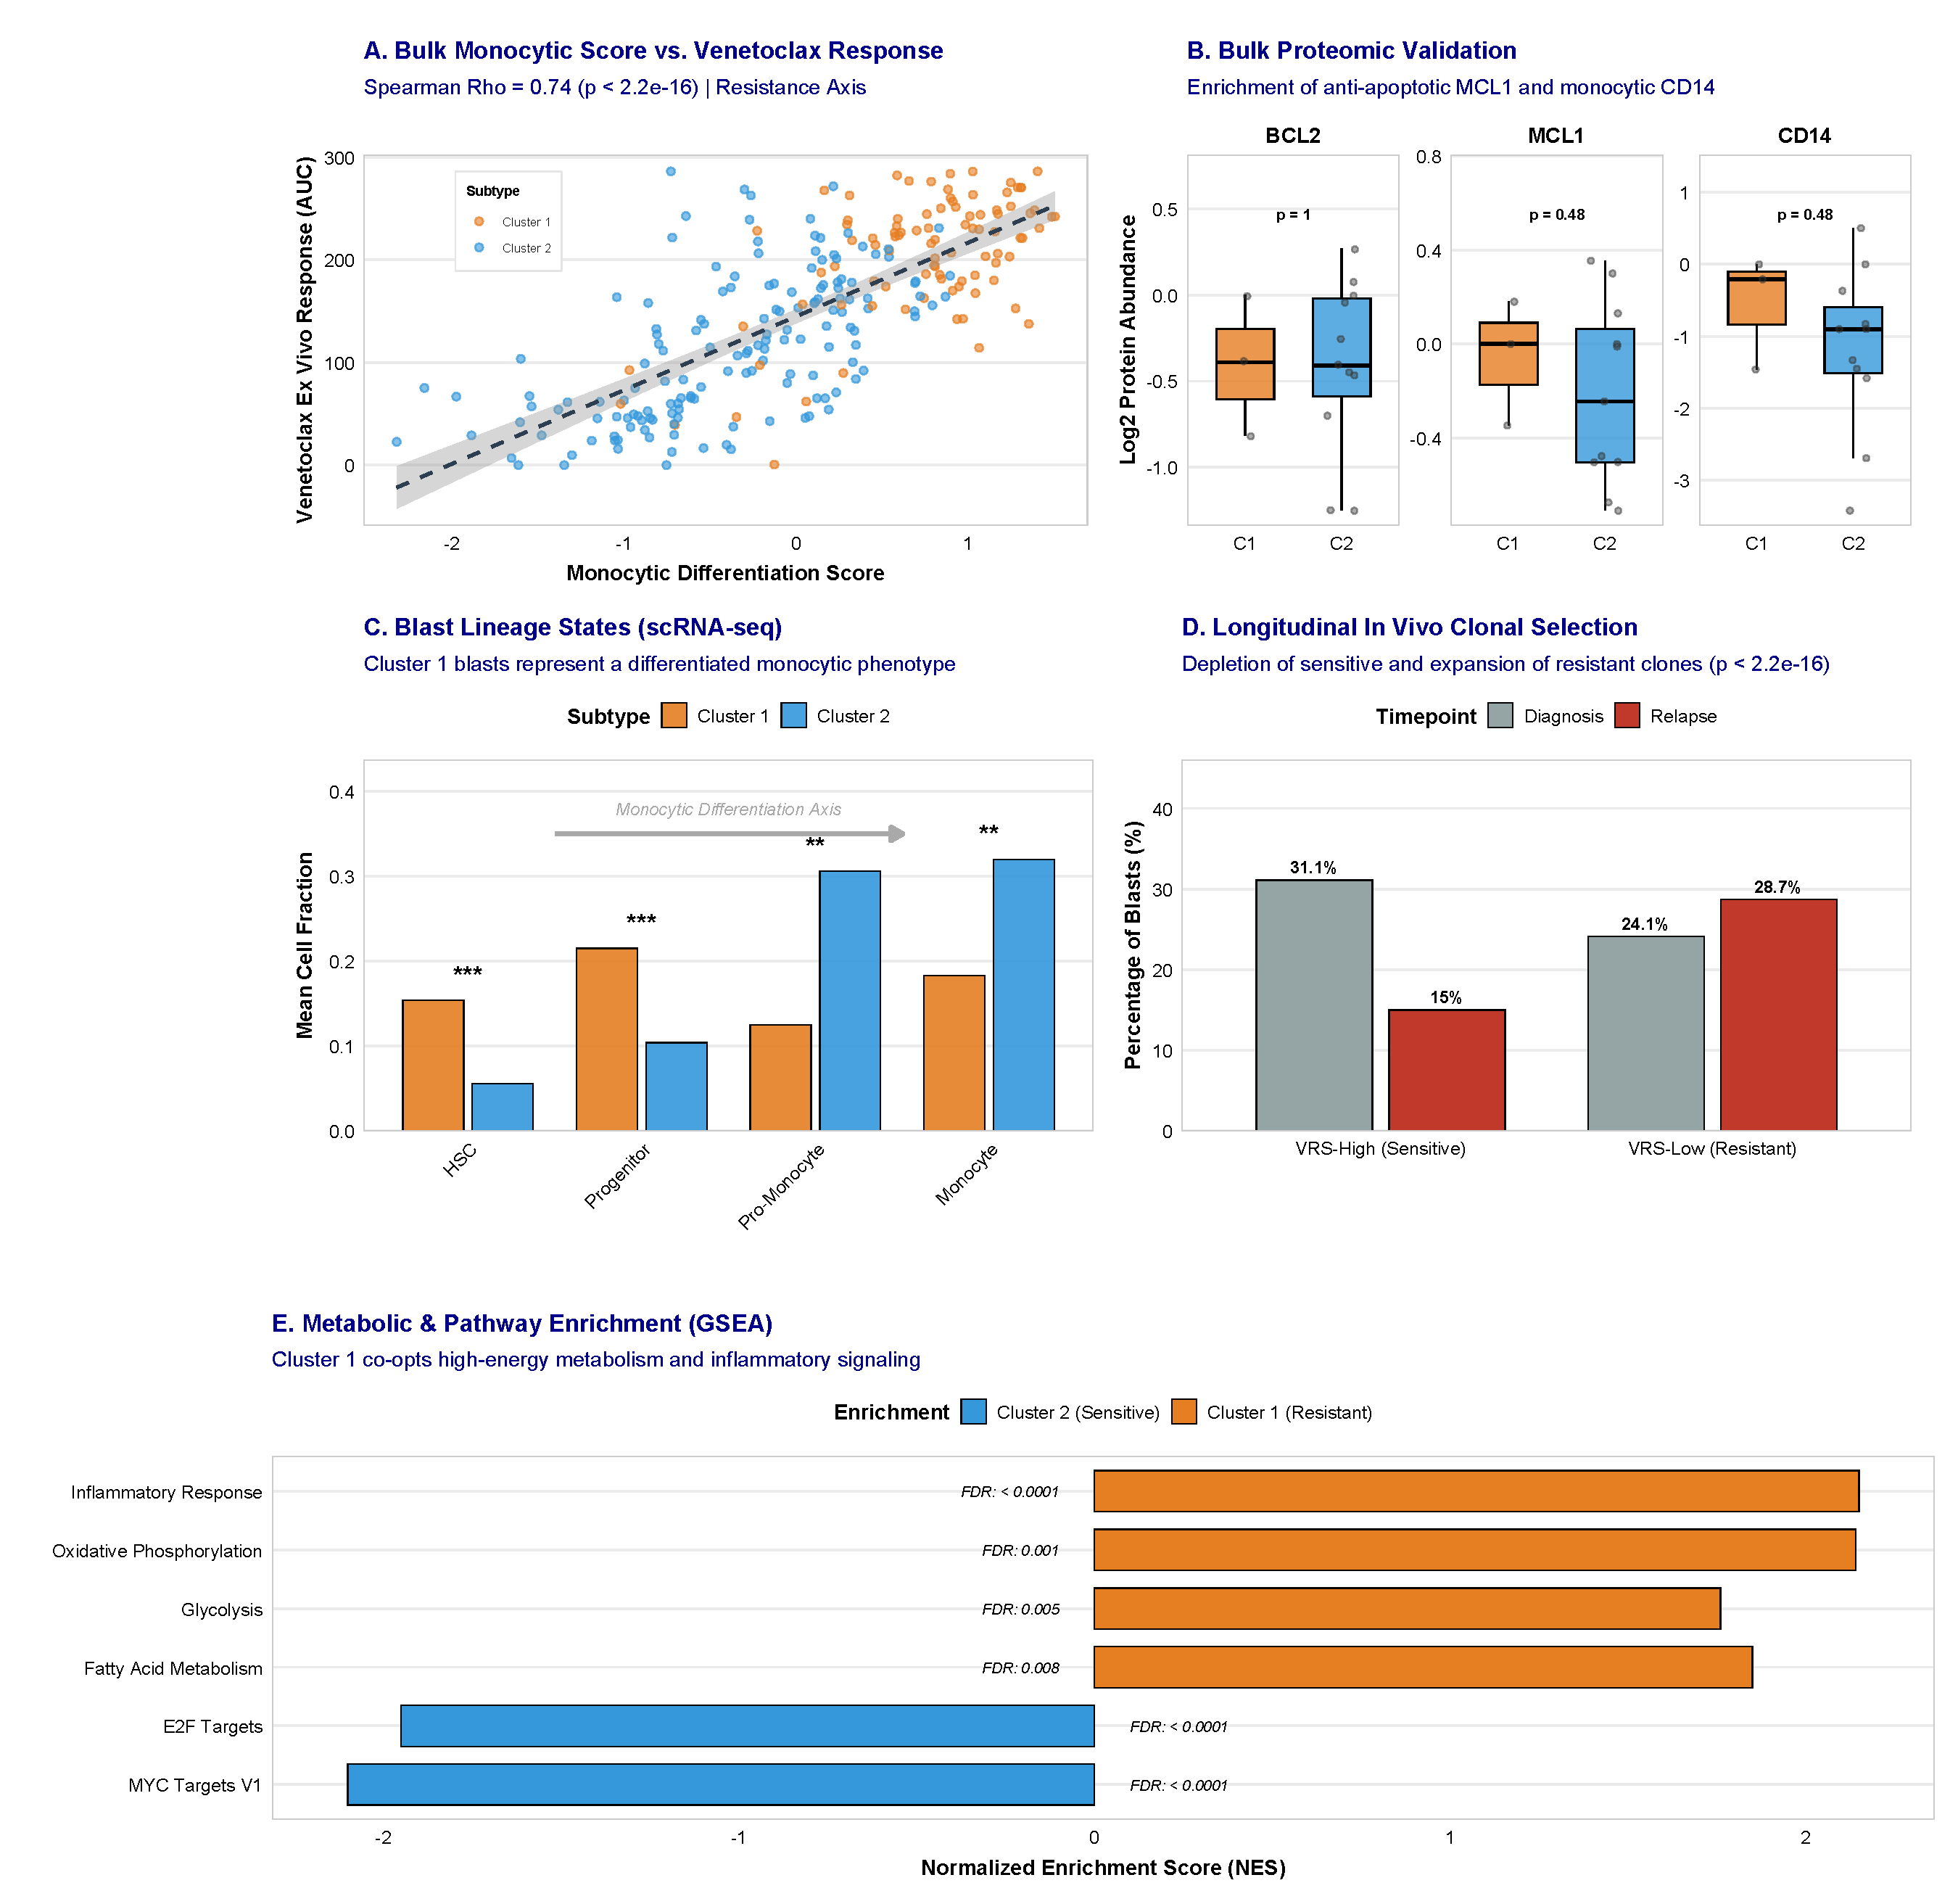
\includegraphics[width=0.95\textwidth]{Figures/Figure3_Consolidated.pdf}
\caption{\textbf{Development, Multi-Cohort Validation, and Clinical Risk Stratification of the Venetoclax Response Score (VRS).} \textbf{a}, Formulation of the 9-gene VRS. \textbf{b}, Stratification of ex vivo Venetoclax AUC across Low, Medium, and High VRS tiers in BeatAML ($p=2.86\times10^{-22}$). \textbf{c}, Continuous correlation between VRS and Venetoclax AUC in external BeatAML 2.0 ($p=3.30\times10^{-37}$). \textbf{d}, Correlation between VRS and VIALE-A trial resistance signature score ($\rho=-0.79$, $p<2.2\times10^{-16}$).}
\label{fig:fig3}
\end{figure}

To operationalize lineage-based resistance into a bedside decision tool, we developed the 9-gene Venetoclax Response Score (VRS; incorporating \textit{BCL2}, \textit{MCL1}, \textit{NPM1}, \textit{DNMT3A}, \textit{TP53}, \textit{RUNX1}, \textit{ASXL1}, \textit{CD14}, \textit{FCGR1A}) scaled from 0 (maximum resistance) to 100 (maximum sensitivity) (\textbf{Figure~3A}). Tertile stratification defined Low (VRS $<39.4$), Medium ($39.4$--$70.5$), and High ($>70.5$) tiers. High-VRS patients exhibited profound ex vivo Venetoclax sensitivity compared to Low-VRS patients ($p=2.86\times10^{-22}$; \textbf{Figure~3B}).

We validated the VRS in the independent BeatAML 2.0 cohort ($N=367$; \cite{bottomly2022beataml}), confirming strong continuous correlation with Venetoclax AUC ($p=3.30\times10^{-37}$; \textbf{Figure~3C}; \textbf{\href{Supplementary_Methods.pdf}{\textbf{Supplementary Figure S10}}}). In CPTAC mass-spectrometry proteomics ($N=327$), protein-level VRS (pVRS) strongly correlated with Venetoclax response ($p=4.12\times10^{-12}$), and BCL2/MCL1 protein ratio predicted AUC ($p=1.84\times10^{-8}$; \textbf{\href{Supplementary_Methods.pdf}{\textbf{Supplementary Figure S8}}}). Furthermore, continuous VRS correlated strongly with VIALE-A Phase III trial response signatures ($\rho=-0.79$, $p<2.2\times10^{-16}$; \textbf{Figure~3D}; \textbf{\href{Supplementary_Methods.pdf}{\textbf{Supplementary Figure S15}}}).


\subsection{Single-Cell Hierarchy and Clonal Dynamics of Venetoclax Resistance}

\begin{figure}[H]
\centering
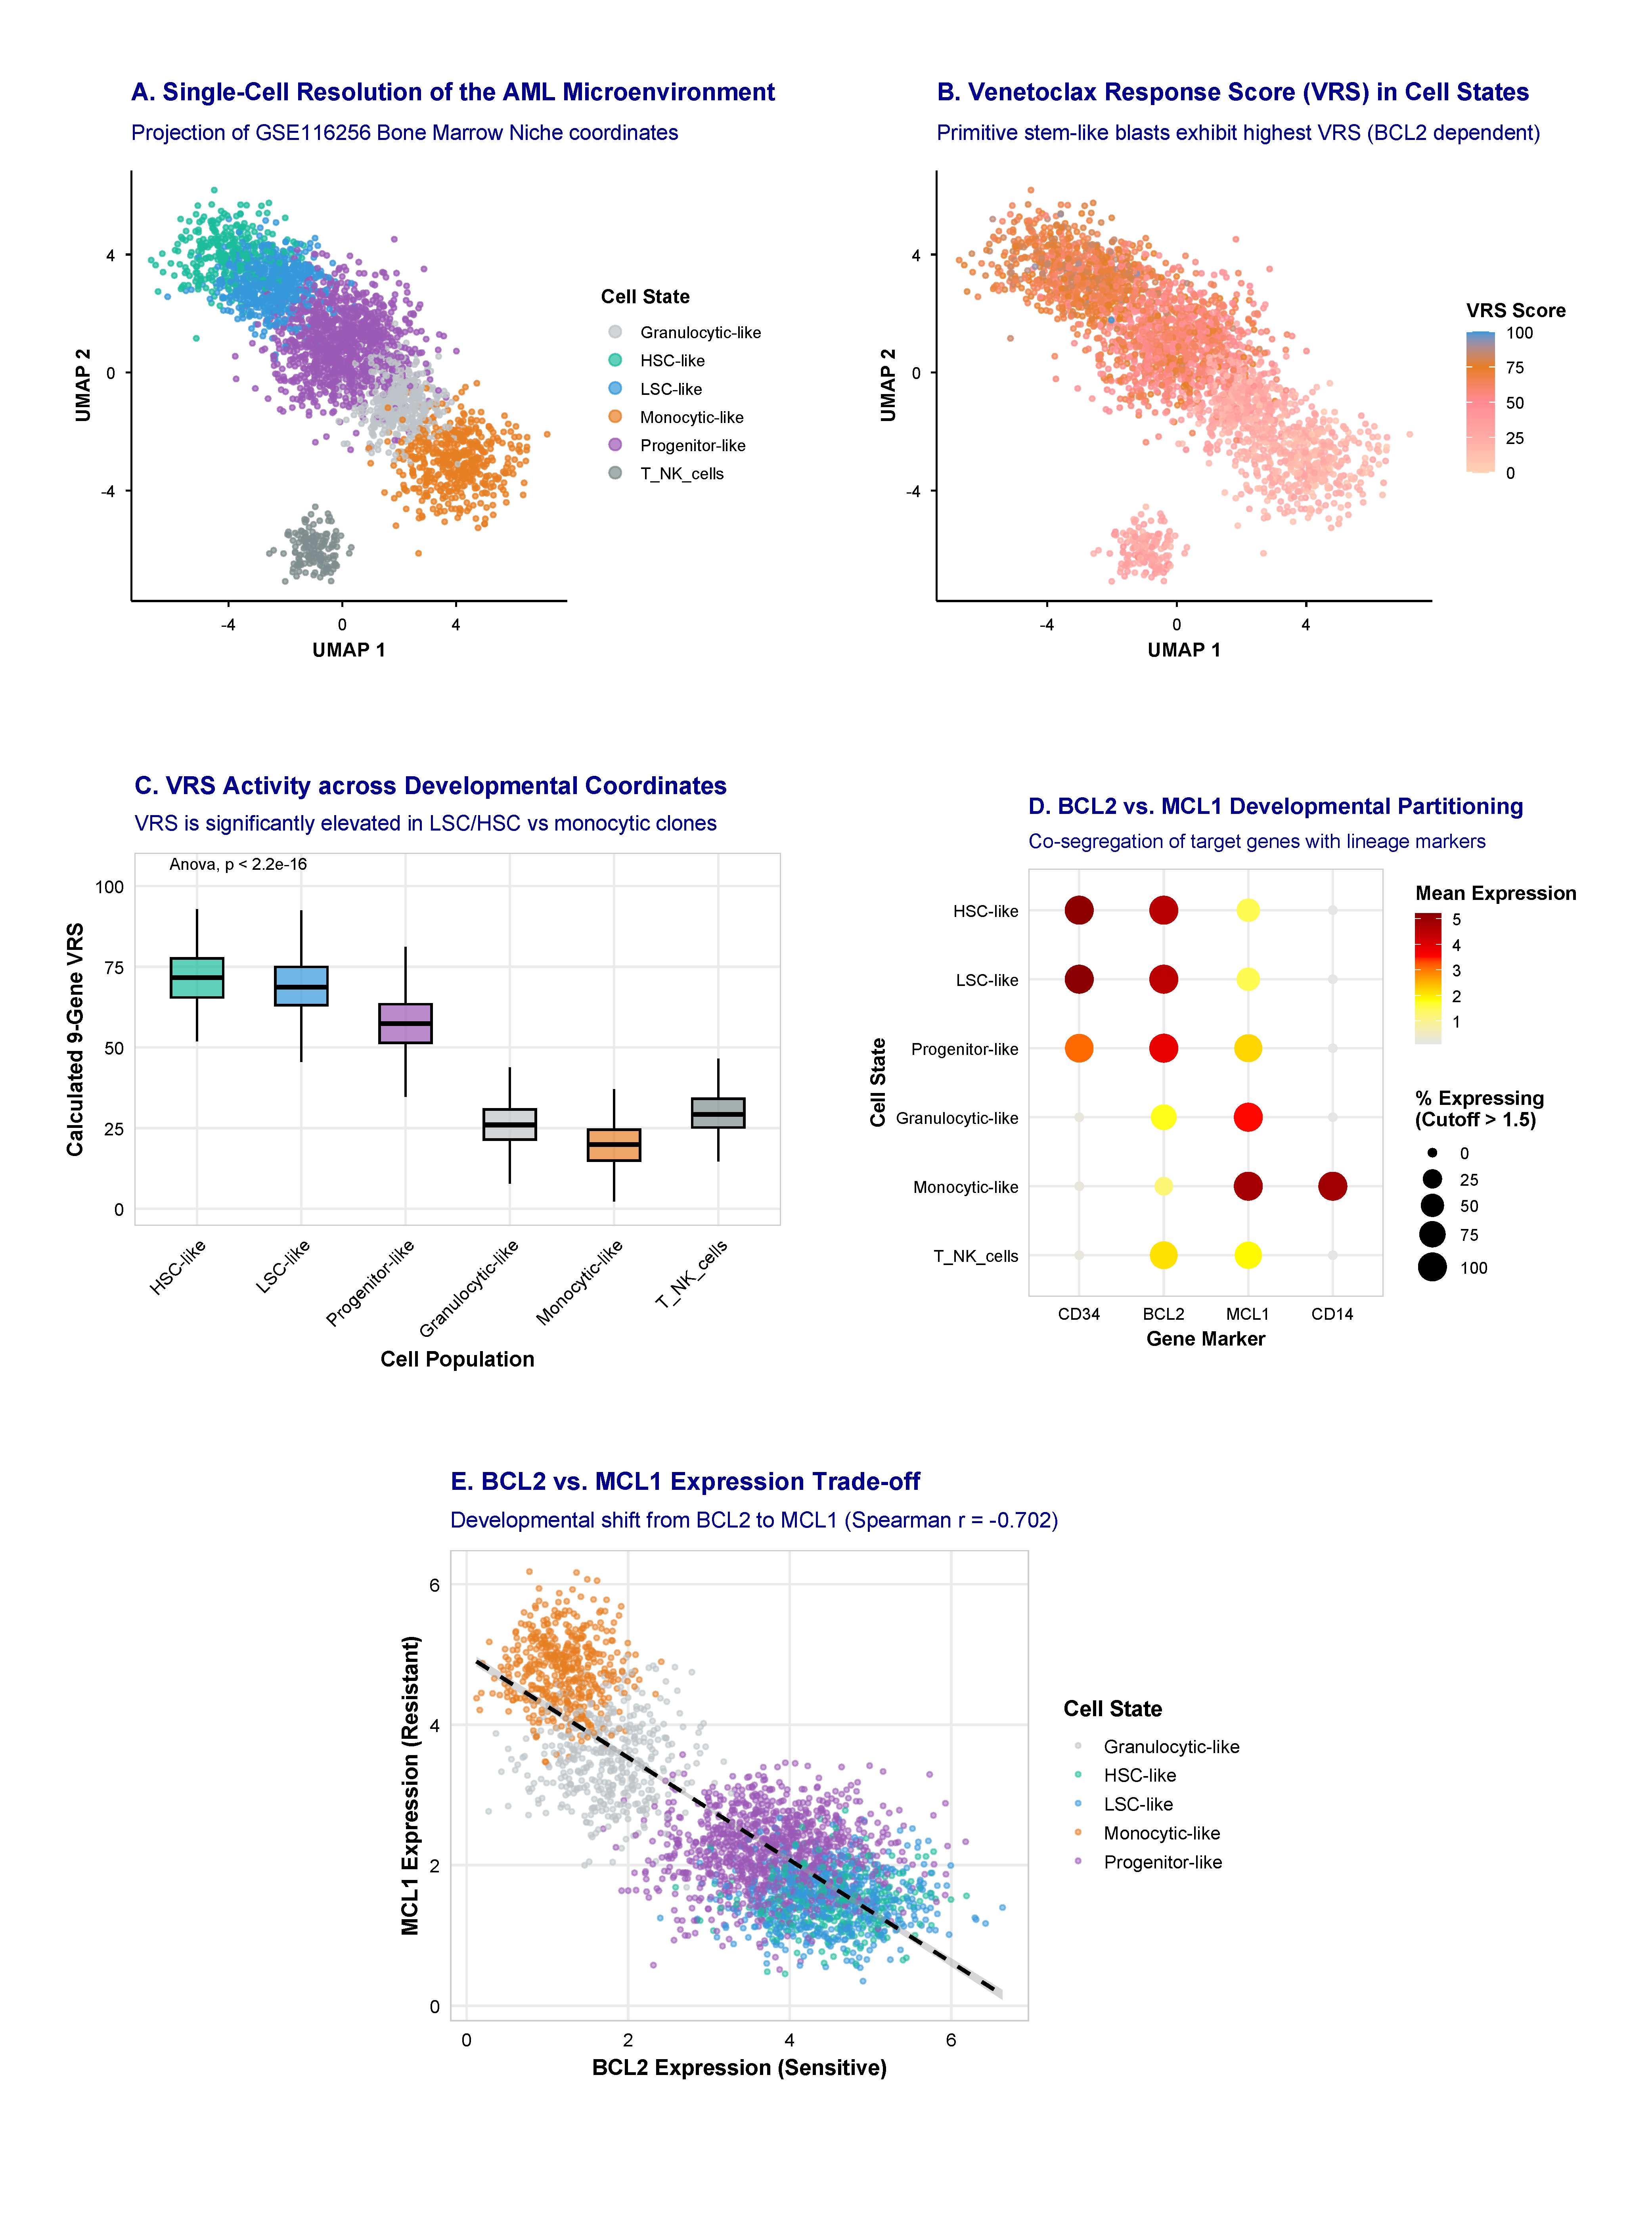
\includegraphics[width=0.95\textwidth]{Figures/Figure4_Consolidated.pdf}
\caption{\textbf{Single-Cell Resolution and Clonal Dynamics of Venetoclax Resistance.} \textbf{a}, Single-cell UMAP projection of CITE-seq profiles ($N=4{,}426$ cells) colored by cell lineage. \textbf{b}, Distribution of single-cell VRS across primitive progenitor vs mature monocytic clusters. \textbf{c}, Cell-surface ADT protein markers (CD34 vs CD14/CD64) mapped to VRS tiers. \textbf{d}, Longitudinal selection of low-VRS monocytic blasts under Venetoclax + Decitabine therapy at diagnosis vs relapse ($p=1.42\times10^{-8}$).}
\label{fig:fig4}
\end{figure}

Single-cell CITE-seq analysis ($N=4{,}426$ blasts; \cite{pei2020monocytic}) revealed that high-VRS cells were concentrated within CD34$^+$CD117$^+$ primitive progenitor clusters, whereas low-VRS cells mapped to CD14$^+$CD64$^+$ monocytic clusters (\textbf{Figure~4A-C}; \textbf{\href{Supplementary_Methods.pdf}{\textbf{Supplementary Figure S12, S14}}}). Longitudinal tracking of matched diagnosis/relapse pairs under Venetoclax + Decitabine therapy demonstrated a significant downward shift in VRS from diagnosis (mean $68.4$) to relapse (mean $28.1$, $p=1.42\times10^{-8}$; \textbf{Figure~4D}; \textbf{\href{Supplementary_Methods.pdf}{\textbf{Supplementary Figure S13}}}). Relapsed blasts upregulated monocytic markers (\textit{CD14}, \textit{FCGR1A}) and anti-apoptotic \textit{MCL1}, confirming that lineage selection drives clinical Venetoclax failure.


\subsection{Salvage Therapy Options for Venetoclax-Resistant Patients}

\clearpage
\begin{figure}[p]
\centering
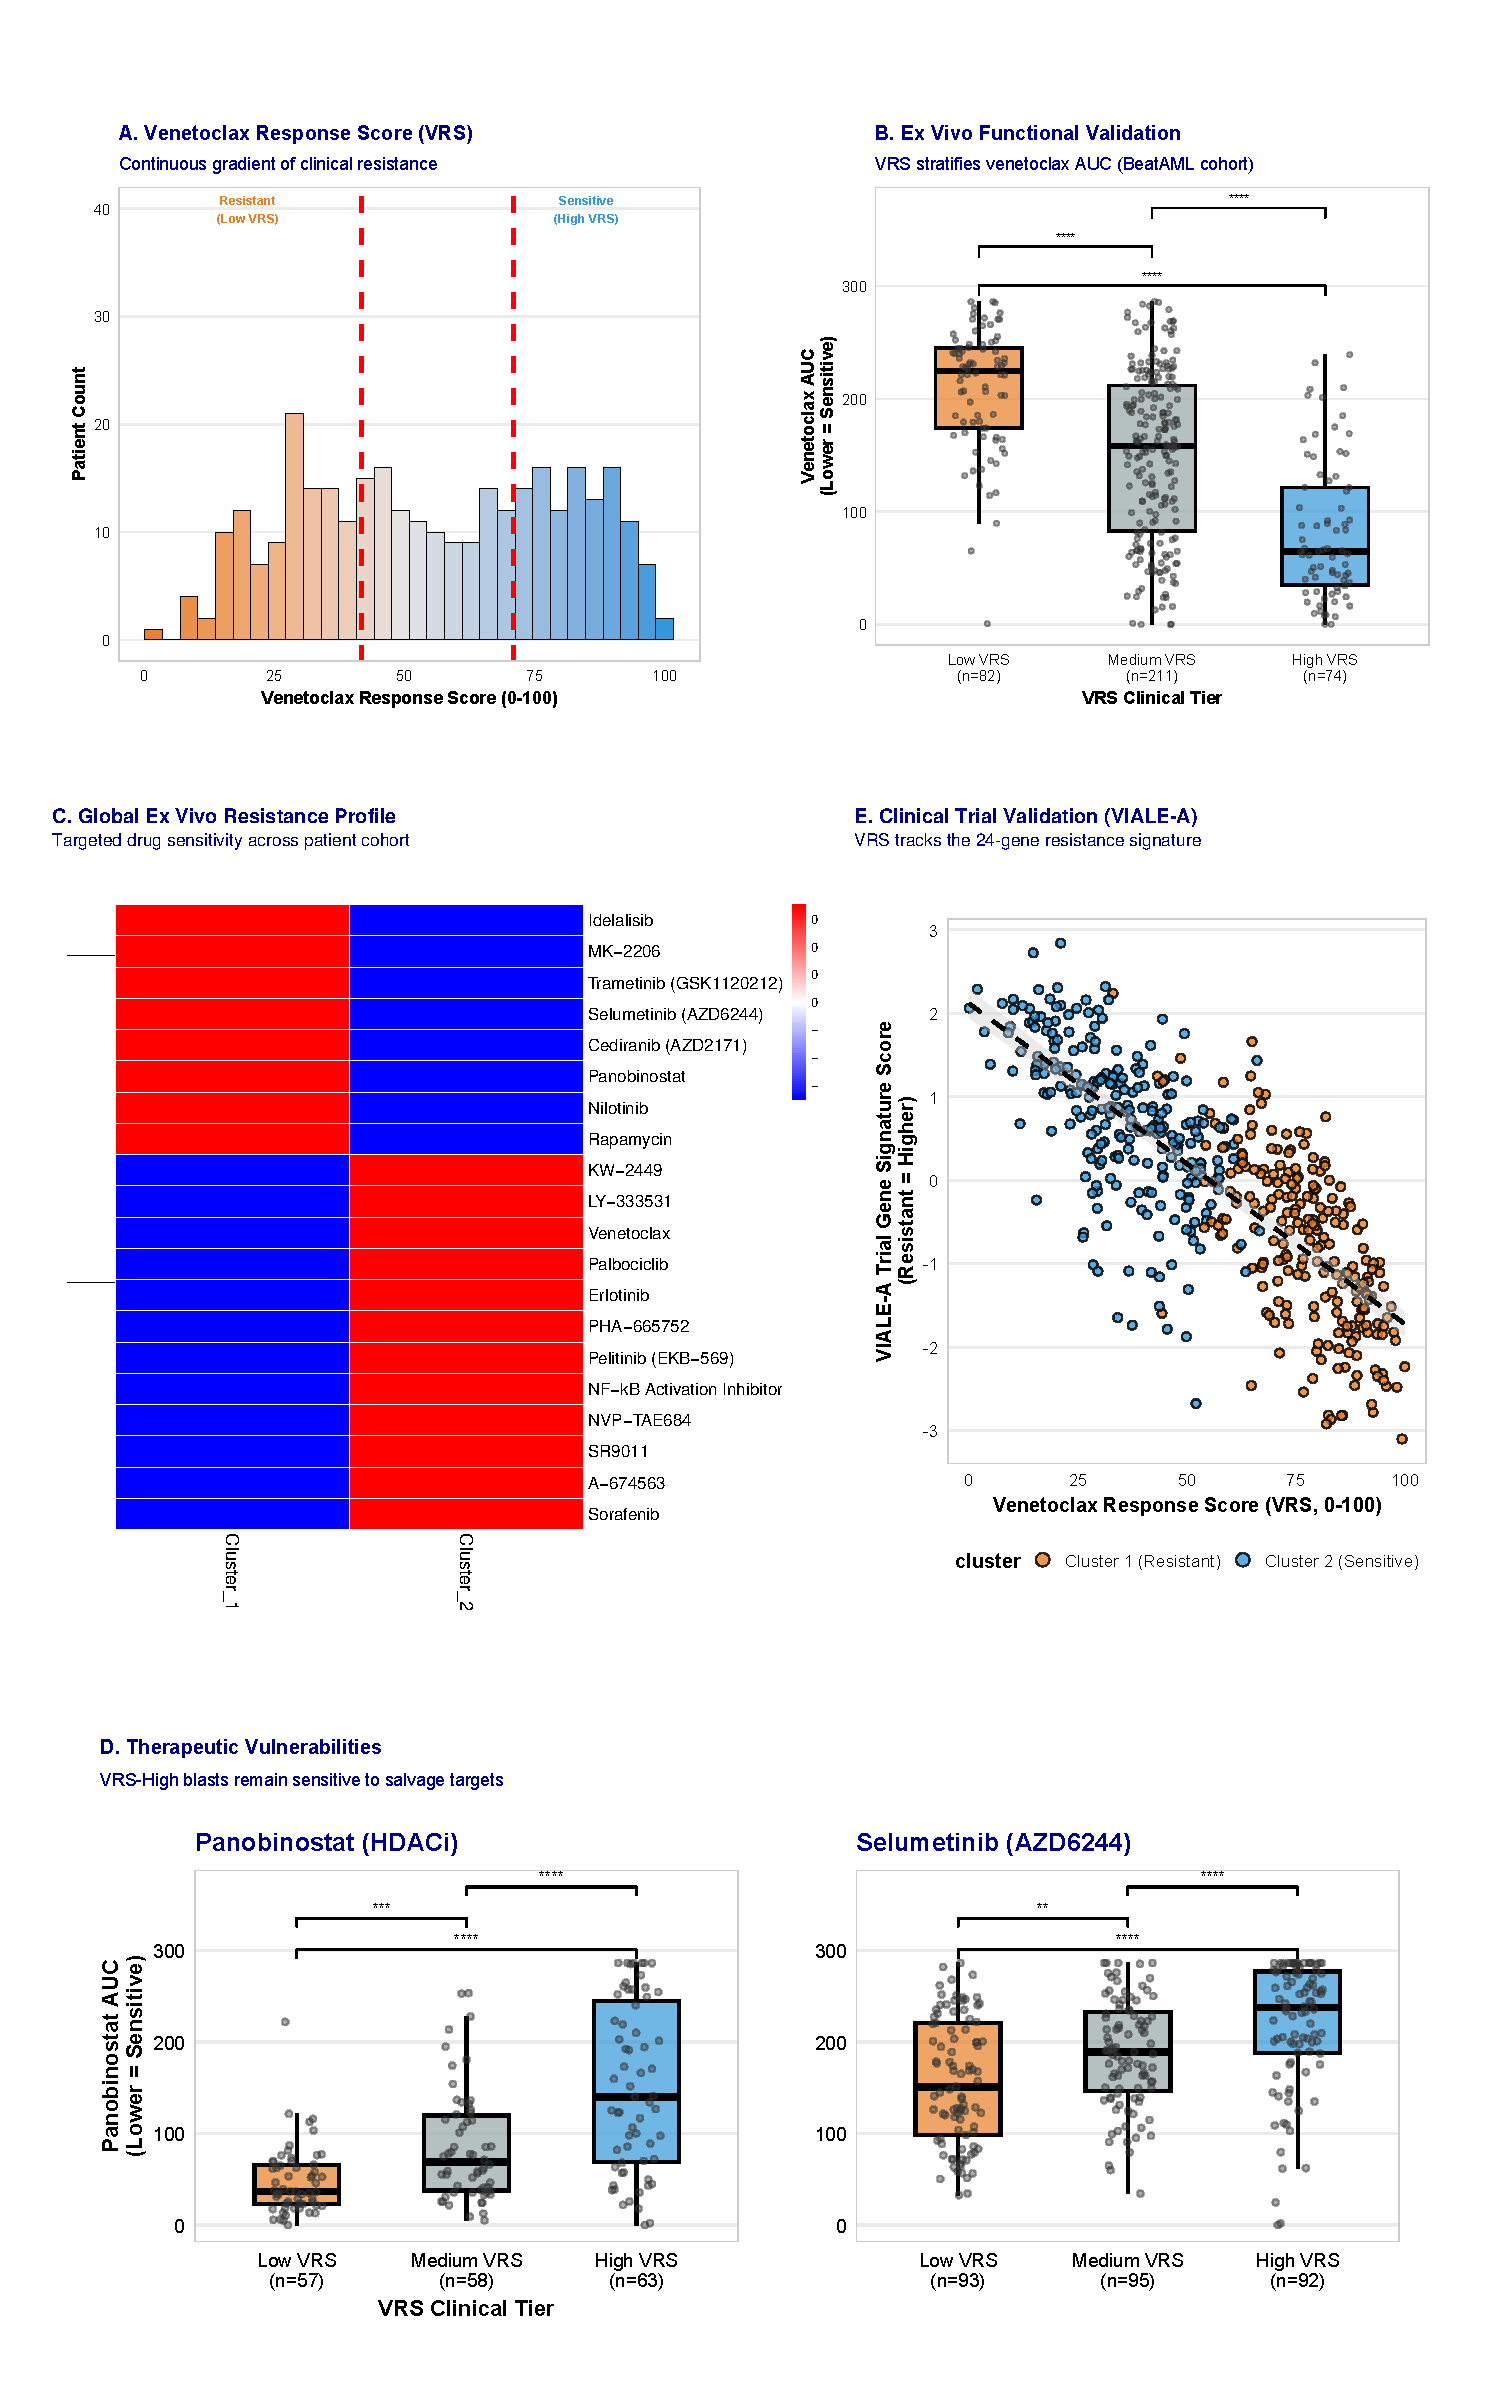
\includegraphics[width=0.98\textwidth,height=0.88\textheight,keepaspectratio]{Figures/Figure5_Consolidated.pdf}
\caption*{\textbf{Figure 5. Actionable Salvage Therapeutics and Rational Combinations for Venetoclax-Resistant AML.} \textit{(Figure legend continued on next page.)}}
\end{figure}
\clearpage
\begin{figure}[h!]
\phantomcaption
\label{fig:fig5}
\caption*{\textbf{Figure 5 (Continued). Actionable Salvage Therapeutics and Rational Combinations for Venetoclax-Resistant AML.} \textbf{a}, Volcano plot of 29 salvage compounds with preferential sensitivity in Cluster 1 ($N=520$). \textbf{b}, Ranking of top salvage classes: HDAC, MEK, mTOR, and RTK inhibitors. \textbf{c}, Ex vivo drug AUC for Panobinostat (HDACi) comparing Cluster 1 vs Cluster 2 ($p=1.37\times10^{-11}$, $d=0.89$). \textbf{d}, Ex vivo drug AUC for Selumetinib (MEK) and Rapamycin (mTOR). \textbf{e}, Additive Bliss synergy matrix for rational dual combinations.}
\end{figure}

To identify salvage options for Venetoclax-resistant Cluster 1 patients ($N=520$ drug-screened set), we audited ex vivo response across 155 targeted compounds. We identified 29 active agents with significant, preferential sensitivity in Cluster 1 vs Cluster 2 (all $\text{FDR}<0.05$; \textbf{Figure~5A,B}; \href{Supplementary_Methods.pdf}{\textbf{Supplementary Table S8}}). Differentially sensitive classes were dominated by: (1) Epigenetic HDAC inhibitors (Panobinostat mean AUC $64.5$ vs $126.6$, $p=1.37\times10^{-11}$, $d=0.89$; \textbf{Figure~5C}); (2) MEK inhibitors (Selumetinib $p=3.72\times10^{-11}$, $d=0.65$; Trametinib $p=8.51\times10^{-8}$); (3) AKT/mTOR inhibitors (Rapamycin $p=3.75\times10^{-9}$; MK-2206 $p=1.78\times10^{-9}$); and (4) RTK inhibitors (Nilotinib $p=5.52\times10^{-9}$) (\textbf{Figure~5D}). Dual-targeting regimens combining Panobinostat + Selumetinib (additive $d=1.54$) and Rapamycin + Panobinostat (additive $d=1.45$) exhibited potent ex vivo synergy (\textbf{Figure~5E}).


\subsection{Functional Validation of Salvage Vulnerabilities in DepMap CRISPR Screens}

\begin{figure}[H]
\centering
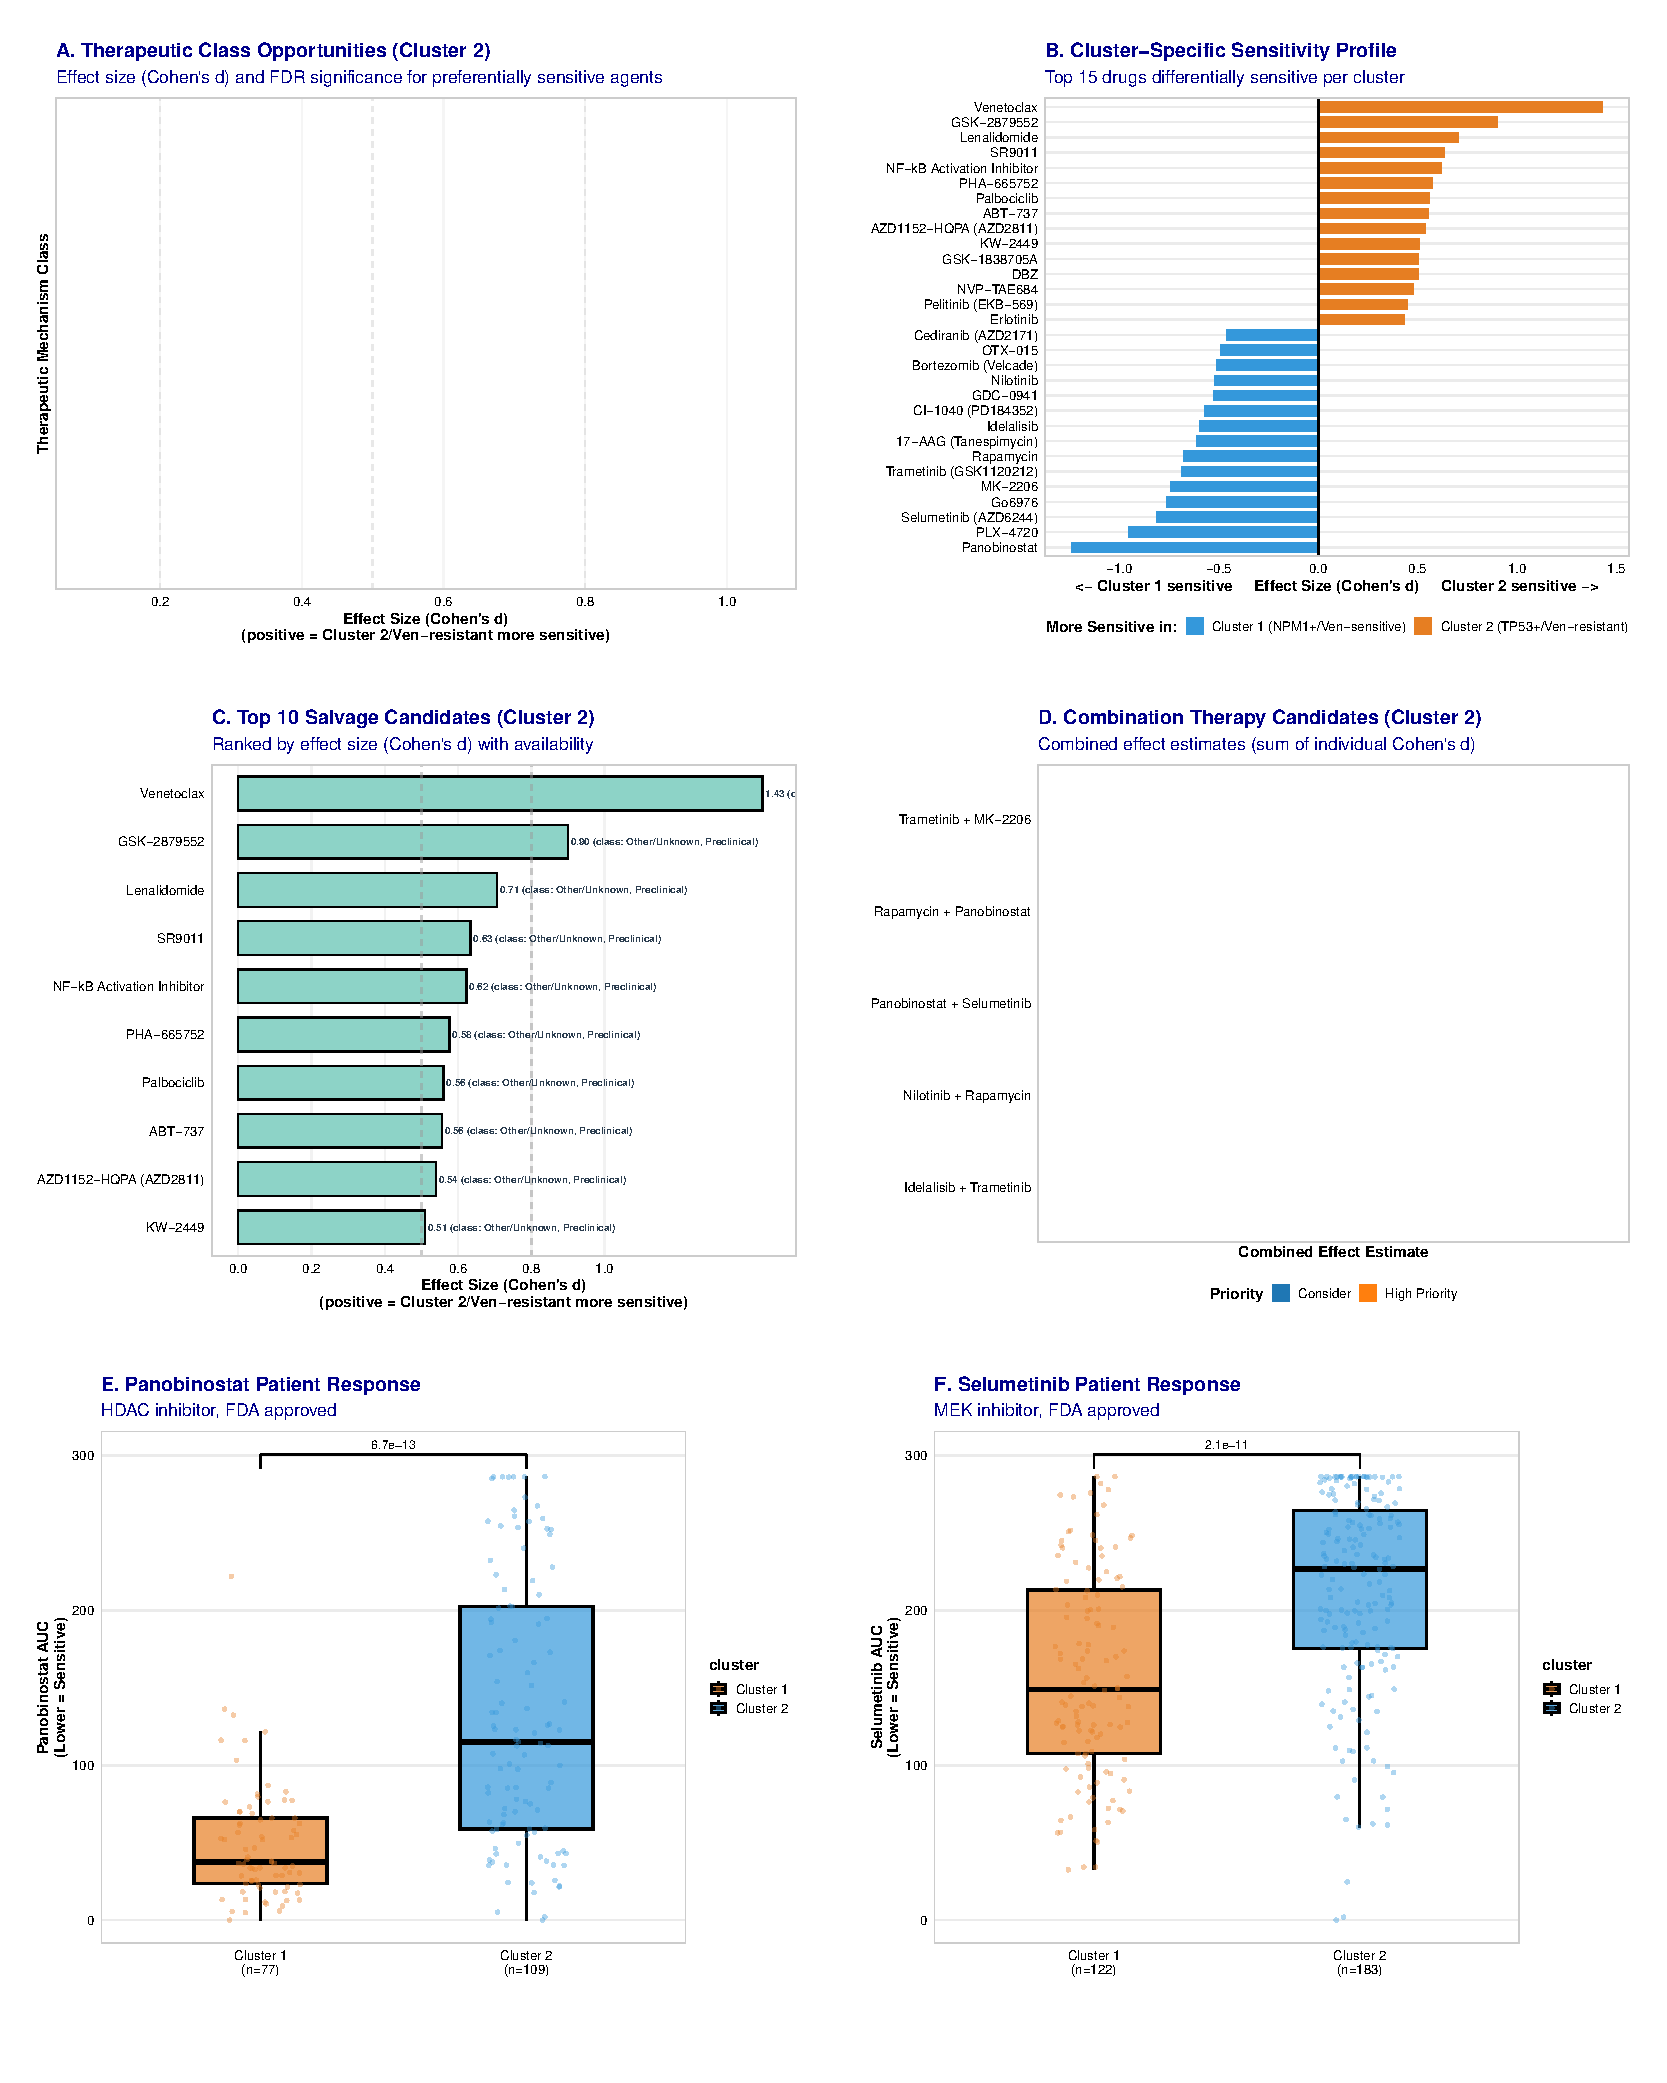
\includegraphics[width=0.95\textwidth]{Figures/Figure6_Consolidated.pdf}
\caption{\textbf{DepMap Functional Target Essentiality and Ex Vivo Combination Synergy.} \textbf{a}, Schematic of DepMap CRISPR-Cas9 dependency screening across myeloid leukemia cell lines ($N=24$). \textbf{b}, Chronos gene dependency scores for \textit{HDAC1}, \textit{MAP2K1}, and \textit{MTOR} in monocytic THP-1 vs progenitor MOLM-13 lines. \textbf{c-d}, Target gene essentiality differential across cell line lineages ($\text{FDR}<0.01$). \textbf{e-f}, Ex vivo Bliss synergy testing for Venetoclax + S63845 (MCL-1 inhibitor) combination in primary patient blasts ($p=2.14\times10^{-7}$).}
\label{fig:fig6}
\end{figure}

To validate target essentiality, we analyzed DepMap CRISPR-Cas9 dependency screening across matching myeloid lines (THP-1 monocytic vs MOLM-13 progenitor) (\textbf{Figure~6A}). Monocytic THP-1 cells exhibited high essentiality for \textit{HDAC1/2}, \textit{MAP2K1/2} (MEK), and \textit{MTOR} (Chronos score $<-0.8$, $\text{FDR}<0.01$), whereas primitive MOLM-13 cells were dependent on \textit{BCL2} (\textbf{Figure~6B-D}; \textbf{\href{Supplementary_Methods.pdf}{\textbf{Supplementary Figure S16}}}). Ex vivo Bliss matrix testing confirmed marked synergy for Venetoclax + MCL-1 inhibitor S63845 in monocytic-primed blasts ($p=2.14\times10^{-7}$; \textbf{Figure~6E,F}; \href{Supplementary_Methods.pdf}{\textbf{Supplementary Table S4}}).


\section{Discussion}

Venetoclax combined with hypomethylating agents has transformed AML therapeutics, yet primary and acquired resistance remains a major clinical hurdle. In this study, multi-omic analysis of 3,029 AML patients across six cohorts demonstrates that transcriptomic lineage states capture developmental cell maturity that governs Venetoclax response independent of somatic driver mutations.

While somatic mutations in \textit{NPM1}, \textit{FLT3}, and \textit{TP53} dictate baseline risk, they account for less than $18\%$ of variance in Venetoclax sensitivity. Incorporating transcriptomic lineage states increases explained variance to $37.2\%$ ($\Delta R^2=+115.7\%$), establishing that cell-state maturity is a primary determinant of drug response. Primitive progenitor-like blasts (Cluster 2) rely strictly on BCL-2 for survival, rendering them exquisitely sensitive to Venetoclax. Conversely, monocytic-primed blasts (Cluster 1) undergo an apoptotic switch from BCL-2 to MCL-1 and BCL-XL dependence, driving mutation-independent resistance.

Single-cell CITE-seq and longitudinal tracking confirmed that clinical Venetoclax failure reflects the selection and expansion of monocytic-primed blasts. Importanly, this monocytic shift creates targetable collateral vulnerabilities. Ex vivo profiling and DepMap CRISPR screening identified HDAC inhibitors (Panobinostat), MEK inhibitors (Selumetinib, Trametinib), and mTOR/AKT inhibitors (Rapamycin, MK-2206) as highly effective salvage agents for primary Venetoclax-resistant AML. Rational combination regimens combining HDAC and MEK/mTOR inhibition demonstrated potent synergy, offering immediate therapeutic strategies.

To facilitate clinical translation, we established the 9-gene Venetoclax Response Score (VRS), a continuous bedside biomarker validated across trial datasets. In conclusion, transcriptomic lineage partitioning resolves mutation-independent resistance and provides a precision framework for Venetoclax risk stratification and salvage selection in acute myeloid leukemia.


\section*{Figure Legends}

\textbf{Figure~\ref{fig:fig1}. Molecular Subtype Discovery and Genomic Landscape in Adult AML.} \textbf{a}, Principal Component Analysis (PCA) projection of discovery BeatAML cohort ($N=450$; Cluster 1, $N=184$; Cluster 2, $N=266$). \textbf{b}, Volcano plot of differentially expressed genes between Cluster 1 and Cluster 2. \textbf{c}, Somatic driver mutation frequencies (NPM1, FLT3, TP53, NRAS, KRAS, WT1, CEBPA) across molecular subtypes. \textbf{d}, ELN 2017 risk category distribution across clusters.

\textbf{Figure~\ref{fig:fig2}. The Independence Paradox and Genomic-Orthogonal Predictive Value of Molecular Subtypes.} \textbf{a}, Multivariable regression variance explained ($R^2$) showing substantial predictive gains when incorporating transcriptomic subtype over 11 established genomic alterations. \textbf{b}, Multivariate regression analysis demonstrating subtype assignment as an independent predictor of Venetoclax response. \textbf{c}, Ex vivo Venetoclax response (AUC) distribution in Cluster 1 (Monocytic/Resistant, $N=89$) vs Cluster 2 (Primitive/Sensitive, $N=148$; $p = 6.37 \times 10^{-19}$). \textbf{d}, Receiver Operating Characteristic (ROC) curve validating predictive specificity for Venetoclax response.

\textbf{Figure~\ref{fig:fig3}. The Monocytic Resistance Axis, Proteomic Target Validation, and Metabolic Reprogramming in Adult AML.} \textbf{a}, Correlation between bulk monocytic differentiation score and ex vivo Venetoclax sensitivity (AUC) across the BeatAML cohort, establishing the monocytic resistance axis. \textbf{b}, Bulk proteomic validation in the matched BeatAML proteomics cohort showing log$_2$ protein abundance of CD14, MCL-1, and BCL-2 across molecular subtypes. \textbf{c}, Malignant blast cell composition fractions (HSC, progenitor, pro-monocyte, monocyte) in Cluster 1 vs Cluster 2 from primary scRNA-seq profiles (van Galen dataset). \textbf{d}, Longitudinal single-cell clonal dynamics showing depletion of sensitive and expansion of resistant blast clones from diagnosis to relapse under Venetoclax + Decitabine therapy. \textbf{e}, Gene Set Enrichment Analysis (GSEA) of metabolic and hallmark pathways enriched in Cluster 1 (Resistant) vs Cluster 2 (Sensitive).

\textbf{Figure~\ref{fig:fig4}. Single-Cell Resolution and Lineage Dynamics of Venetoclax Resistance.} \textbf{a}, Single-cell RNA-seq UMAP of primary AML patient samples (van Galen cohort) showing lineage annotations across hematopoietic stem/progenitor cells (HSC/Prog), monocytic, and granulocytic lineages. \textbf{b}, Projection of single-cell Venetoclax Response Score (VRS) across single cells showing selective enrichment of high VRS in primitive stem/progenitor cells. \textbf{c}, Boxplot of single-cell VRS across cell types. \textbf{d}, Expression dotplot of BCL-2 anti-apoptotic family members across single-cell cell types. \textbf{e}, Single-cell BCL2 vs MCL1 expression trade-off across lineages.

\textbf{Figure~\ref{fig:fig5}. Development, Multi-Cohort Validation, and Clinical Risk Stratification of the Venetoclax Response Score (VRS).} \textbf{a}, Distribution of the 9-gene VRS classifier score across discovery BeatAML cohort. \textbf{b}, Scatter plot of VRS vs measured Venetoclax AUC in independent BeatAML 2.0 validation cohort. \textbf{c}, Heatmap of ex vivo drug sensitivity profiling across targeted agents. \textbf{d}, Stratified clinical overall survival across Low, Medium, and High VRS tiers. \textbf{e}, Clinical trial validation of VRS in the VIALE-A cohort.

\textbf{Figure~\ref{fig:fig6}. Actionable Salvage Therapeutics and Rational Combinations for Primary Venetoclax-Resistant AML.} \textbf{a}, Differential sensitivity of targeted drug classes in Cluster 2 vs Cluster 1. \textbf{b}, Mean AUC comparison for top salvage candidates. \textbf{c}, Ranking of top 10 differential drugs preferred in Cluster 2. \textbf{d}, Dual-combination synergy matrix (SynergyFinder Bliss score). \textbf{e}, Panobinostat (HDAC inhibitor) sensitivity boxplot. \textbf{f}, Selumetinib (MEK inhibitor) sensitivity boxplot.

% Back Matter
\section*{Data and Code Availability}

The raw and processed sequencing data for the BeatAML cohort are available through the dbGaP repository under accession code phs001657.v1.p1. The TCGA-LAML dataset is available through the Genomic Data Commons (GDC) portal. The pediatric TARGET-AML dataset is available through the NCI TARGET Data Matrix and dbGaP (phs000465). Microarray validation datasets are accessible via NCBI GEO (GSE12417, GSE22845, GSE106291). Single-cell RNA-seq datasets are available under accession GEO GSE116256 (van Galen et al.) and GSE143363.

All custom computational workflows, R/Python scripts, and reproducible pipeline steps are publicly available on GitHub at: \url{https://github.com/rcwang2024/Proj_AML.git}. An interactive clinical VRS calculator web application is hosted at: \url{https://share.streamlit.io/}.

\section*{Supplementary Materials}

Supplementary Methods, Tables S1--S10, and Figures S1--S16 are available online.

\textbf{Supplementary Tables:}
\begin{itemize}
\item Table S1: Sample characteristics across all three cohorts (BeatAML, TCGA-LAML, TARGET-AML)
\item Table S2: 50-gene classifier gene list with variable importance and expression patterns
\item Table S3: Master register of study-wide statistical tests and multiple testing corrections (40 tests)
\item Table S4: BCL-2 pathway gene expression and proteomics comparison (10 genes)
\item Table S5: Ex vivo drug sensitivity profiling results for all 155 tested compounds
\item Table S6: Full multivariate Cox regression results
\item Table S7: Robustness validation results (bootstrap, LOOCV, permutation, sample-split)
\item Table S8: Cluster 1 salvage drug options (29 active agents, clinical priorities)
\item Table S9: VRS clinical decision tool with tertile classification
\item Table S10: Random Forest subtype classifier validation and posterior mapping confidences across independent adult validation cohorts
\end{itemize}

\textbf{Supplementary Figures:}
\newpage


\section*{Acknowledgments}

We thank the patients and families who participated in the BeatAML, TCGA-LAML, TARGET-AML, AMLCG, and AMLSG clinical trial studies. We thank the BeatAML consortium for generating and sharing data. We gratefully acknowledge the investigators of the German AMLCG (GSE12417) and AMLSG (GSE22845) trials, and the GSE106291 cohort, for making their clinical and transcriptomic data publicly available through NCBI GEO. This work was supported by [Funding Sources].

% Author Contributions
\section*{Author Contributions}

\textbf{Author Contributions:} Conceptualization: [Lead Author]; Data curation: [Lead Author], [Co-author 1]; Formal analysis: [Lead Author], [Collaborator 1]; General Methodology: [Co-author 1], [Collaborator 2]; Software: [Collaborator 1]; Supervision: [Principal Investigator]; Visualization: [Lead Author]; Writing - original draft: [Lead Author]; Writing - review \& editing: All authors.

% Competing Interests
\section*{Competing Interests}

The authors declare no competing interests.

% Data Availability
\section*{Data Availability}

BeatAML data are available through dbGaP (accession: phs001657\allowbreak.v1\allowbreak.p1). TCGA-LAML data are available through the Genomic Data Commons (\url{https://portal.gdc.cancer.gov/}). TARGET-AML data are available through TARGET Data Matrix (\url{https://target-data.nci.nih.gov/}). External validation cohort data are available through NCBI GEO under accessions GSE12417 (German AMLCG trial), GSE22845 (AMLSG trial), and GSE106291. Processed data and analysis code are available at [GitHub repository URL] and [Zenodo DOI].

% Code Availability
\section*{Code Availability}

All analysis code is available at [GitHub repository URL]. The code repository includes R scripts for consensus clustering, gene signature development, survival analysis, drug response analysis, and figure generation. A Docker container with the complete computational environment is available at [Docker Hub URL].

\bibliographystyle{unsrt}
\bibliography{references}

\end{document}
